\documentclass{beamer}

\input{settings.tex}


\title{Algebra on two dimensions}
\subtitle{Math and modeling for high school, Lecture 2}
\author{by Sergei Savin}
\centering
\date{Fall 2022}



\begin{document}
\maketitle


%\begin{frame}{Content}
%
%\begin{itemize}
%\item Motivation
%\item Ordinary differential equations
%    \begin{itemize}
%    \item 1st order
%    \item n-th order
%    \end{itemize}
%\item Linear differential equations
%    \begin{itemize}
%    \item 1st order
%    \item n-th order
%    \end{itemize}
%\item Changing n-th order ODE to a State-Space form
%\item State-Space to ODE
%\item Read more
%\end{itemize}
%
%\end{frame}





\begin{frame}{Linear graphs}
	% \framesubtitle{Part 1}
	\begin{flushleft}
		




\tikzset{every picture/.style={line width=0.75pt}} %set default line width to 0.75pt        

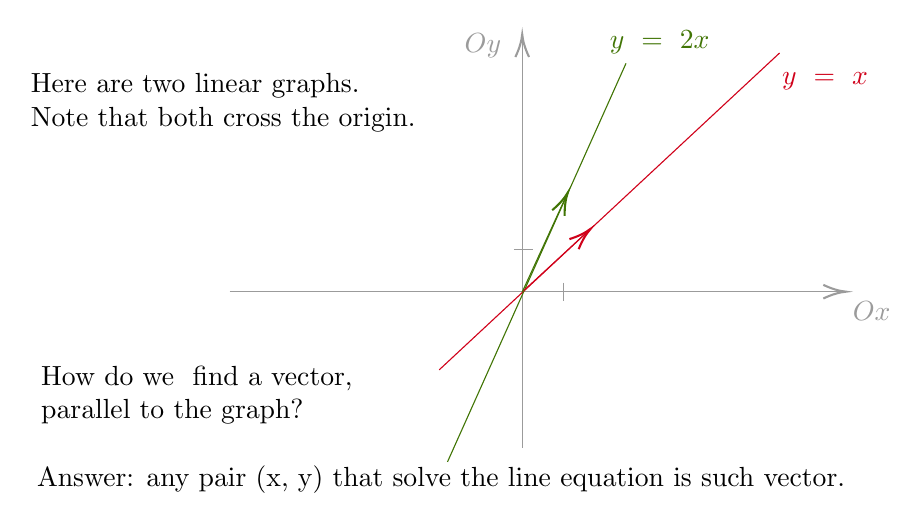
\begin{tikzpicture}[x=0.75pt,y=0.75pt,yscale=-1,xscale=1]
	%uncomment if require: \path (0,300); %set diagram left start at 0, and has height of 300
	
	%Straight Lines [id:da03963288748552296] 
	\draw [color={rgb, 255:red, 155; green, 155; blue, 155 }  ,draw opacity=1 ]   (260,205.5) -- (260,8.33) ;
	\draw [shift={(260,6.33)}, rotate = 90] [color={rgb, 255:red, 155; green, 155; blue, 155 }  ,draw opacity=1 ][line width=0.75]    (10.93,-3.29) .. controls (6.95,-1.4) and (3.31,-0.3) .. (0,0) .. controls (3.31,0.3) and (6.95,1.4) .. (10.93,3.29)   ;
	%Straight Lines [id:da9898822166885091] 
	\draw [color={rgb, 255:red, 155; green, 155; blue, 155 }  ,draw opacity=1 ]   (119,130.33) -- (414,130.33) ;
	\draw [shift={(416,130.33)}, rotate = 180] [color={rgb, 255:red, 155; green, 155; blue, 155 }  ,draw opacity=1 ][line width=0.75]    (10.93,-3.29) .. controls (6.95,-1.4) and (3.31,-0.3) .. (0,0) .. controls (3.31,0.3) and (6.95,1.4) .. (10.93,3.29)   ;
	%Straight Lines [id:da1995149828845848] 
	\draw [color={rgb, 255:red, 208; green, 2; blue, 27 }  ,draw opacity=1 ]   (220,168) -- (384,15.33) ;
	%Straight Lines [id:da3869698901050138] 
	\draw [color={rgb, 255:red, 65; green, 117; blue, 5 }  ,draw opacity=1 ]   (224,212.33) -- (310,20.33) ;
	%Straight Lines [id:da1919377633607524] 
	\draw [color={rgb, 255:red, 155; green, 155; blue, 155 }  ,draw opacity=1 ]   (256,110) -- (265,110) ;
	%Straight Lines [id:da10953300738059357] 
	\draw [color={rgb, 255:red, 155; green, 155; blue, 155 }  ,draw opacity=1 ]   (280,126) -- (280,135) ;
	%Straight Lines [id:da23550777917390864] 
	\draw [color={rgb, 255:red, 208; green, 2; blue, 27 }  ,draw opacity=1 ]   (260,130.5) -- (291.53,101.36) ;
	\draw [shift={(293,100)}, rotate = 137.25] [color={rgb, 255:red, 208; green, 2; blue, 27 }  ,draw opacity=1 ][line width=0.75]    (10.93,-3.29) .. controls (6.95,-1.4) and (3.31,-0.3) .. (0,0) .. controls (3.31,0.3) and (6.95,1.4) .. (10.93,3.29)   ;
	%Straight Lines [id:da2310422637940801] 
	\draw [color={rgb, 255:red, 65; green, 117; blue, 5 }  ,draw opacity=1 ]   (260,130.5) -- (281.17,84.32) ;
	\draw [shift={(282,82.5)}, rotate = 114.62] [color={rgb, 255:red, 65; green, 117; blue, 5 }  ,draw opacity=1 ][line width=0.75]    (10.93,-3.29) .. controls (6.95,-1.4) and (3.31,-0.3) .. (0,0) .. controls (3.31,0.3) and (6.95,1.4) .. (10.93,3.29)   ;
	
	% Text Node
	\draw (384,23.4) node [anchor=north west][inner sep=0.75pt]  [color={rgb, 255:red, 208; green, 2; blue, 27 }  ,opacity=1 ]  {$y\ =\ x$};
	% Text Node
	\draw (301,3.4) node [anchor=north west][inner sep=0.75pt]  [color={rgb, 255:red, 65; green, 117; blue, 5 }  ,opacity=1 ]  {$y\ =\ 2x$};
	% Text Node
	\draw (418,133.73) node [anchor=north west][inner sep=0.75pt]  [color={rgb, 255:red, 155; green, 155; blue, 155 }  ,opacity=1 ]  {$Ox$};
	% Text Node
	\draw (231,4.73) node [anchor=north west][inner sep=0.75pt]  [color={rgb, 255:red, 155; green, 155; blue, 155 }  ,opacity=1 ]  {$Oy$};
	% Text Node
	\draw (22,24) node [anchor=north west][inner sep=0.75pt]   [align=left] {Here are two linear graphs.\\Note that both cross the origin.};
	% Text Node
	\draw (27,165) node [anchor=north west][inner sep=0.75pt]   [align=left] {How do we \ find a vector, \ \\parallel to the graph?};
	% Text Node
	\draw (25,213) node [anchor=north west][inner sep=0.75pt]   [align=left] {Answer: any pair (x, y) that solve the line equation is such vector.};
	
	
\end{tikzpicture}
	
	
		
	\end{flushleft}
\end{frame}



\begin{frame}{Linear graphs}
	% \framesubtitle{Part 1}
	\begin{flushleft}
		
		Example: consider line $y = -3x$. The following vectors line on that line: $(1, \ -3)$, $(-1, \ 3)$, $(3, \ -9)$, etc. In more standard vector notation they are:
		
		\begin{equation}
			\bo{r} =
			\begin{bmatrix}
				1  \\
				-3
			\end{bmatrix}, \ \ 
		\bo{r} =
		\begin{bmatrix}
			-1  \\
			3
		\end{bmatrix}, \ \ 
	\bo{r} =
		\begin{bmatrix}
		3  \\
		-9
		\end{bmatrix}
		\end{equation}
	
	\bigskip
		
		Note that scaling a vector does not change the fact that it lines on the line: if $\bo{r} =
			\begin{bmatrix}
				r_x  \\
				r_y
			\end{bmatrix}$ lies on a line $\mathcal{L}$, than $\lambda \bo{r}$ also lies on $\mathcal{L}$ (where $\lambda \in \mathbb{R}$).
		
		
	\end{flushleft}
\end{frame}


\begin{frame}{Linear graphs}
	% \framesubtitle{Part 1}
	\begin{flushleft}
		
		In fact, we can say the following about a line:
		
		\begin{theorem}
			If $\bo{r} =
			\begin{bmatrix}
				r_x  \\
				r_y
			\end{bmatrix}$ lies on a line $\mathcal{L}$, then all points on $\mathcal{L}$ can be found as $\lambda \bo{r}$.
		\end{theorem}
	
		\bigskip
		
		Let us prove it. If $\mathcal{L} = \{(x, y): \ y = a x \}$ and $\bo{r} \in \mathcal{L}$, then $r_y = a r_x$. Then $\lambda r_y = \lambda a r_x$ and $(\lambda r_x, \lambda r_y) \in \mathcal{L}$. \qed
		
		
	\end{flushleft}
\end{frame}






\begin{frame}{Linear graphs}
	% \framesubtitle{Part 1}
	\begin{flushleft}
		
		That was difficult-looking. But graphically, the proof is quite obvious. We are trying to prove that any point in the line can be reached by scaling the vector lying on that line:
		
		\bigskip
		
		
		\tikzset{every picture/.style={line width=0.75pt}} %set default line width to 0.75pt        
		
		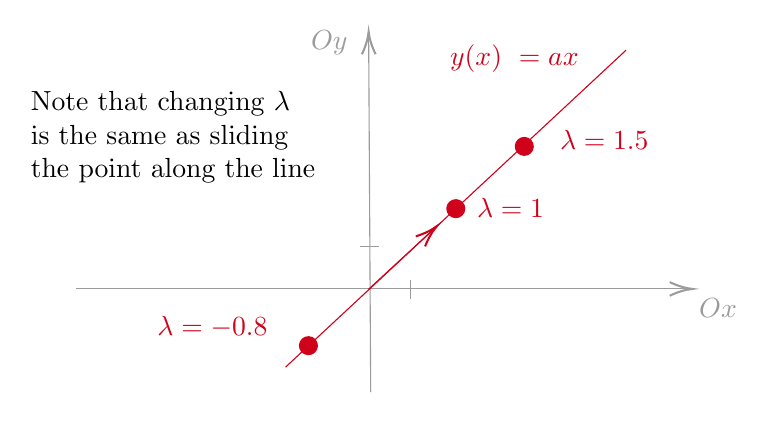
\begin{tikzpicture}[x=0.75pt,y=0.75pt,yscale=-1,xscale=1]
			%uncomment if require: \path (0,300); %set diagram left start at 0, and has height of 300
			
			%Straight Lines [id:da6775811141993964] 
			\draw [color={rgb, 255:red, 155; green, 155; blue, 155 }  ,draw opacity=1 ]   (261,180) -- (260.01,8.33) ;
			\draw [shift={(260,6.33)}, rotate = 89.67] [color={rgb, 255:red, 155; green, 155; blue, 155 }  ,draw opacity=1 ][line width=0.75]    (10.93,-3.29) .. controls (6.95,-1.4) and (3.31,-0.3) .. (0,0) .. controls (3.31,0.3) and (6.95,1.4) .. (10.93,3.29)   ;
			%Straight Lines [id:da12226774606938573] 
			\draw [color={rgb, 255:red, 155; green, 155; blue, 155 }  ,draw opacity=1 ]   (119,130.33) -- (414,130.33) ;
			\draw [shift={(416,130.33)}, rotate = 180] [color={rgb, 255:red, 155; green, 155; blue, 155 }  ,draw opacity=1 ][line width=0.75]    (10.93,-3.29) .. controls (6.95,-1.4) and (3.31,-0.3) .. (0,0) .. controls (3.31,0.3) and (6.95,1.4) .. (10.93,3.29)   ;
			%Straight Lines [id:da8184236755840784] 
			\draw [color={rgb, 255:red, 208; green, 2; blue, 27 }  ,draw opacity=1 ]   (220,168) -- (384,15.33) ;
			%Straight Lines [id:da08056521316880905] 
			\draw [color={rgb, 255:red, 155; green, 155; blue, 155 }  ,draw opacity=1 ]   (256,110) -- (265,110) ;
			%Straight Lines [id:da8358712166652711] 
			\draw [color={rgb, 255:red, 155; green, 155; blue, 155 }  ,draw opacity=1 ]   (280,126) -- (280,135) ;
			%Straight Lines [id:da8358540630991103] 
			\draw [color={rgb, 255:red, 208; green, 2; blue, 27 }  ,draw opacity=1 ]   (260,130.5) -- (291.53,101.36) ;
			\draw [shift={(293,100)}, rotate = 137.25] [color={rgb, 255:red, 208; green, 2; blue, 27 }  ,draw opacity=1 ][line width=0.75]    (10.93,-3.29) .. controls (6.95,-1.4) and (3.31,-0.3) .. (0,0) .. controls (3.31,0.3) and (6.95,1.4) .. (10.93,3.29)   ;
			%Shape: Circle [id:dp12403298271857865] 
			\draw  [color={rgb, 255:red, 208; green, 2; blue, 27 }  ,draw opacity=1 ][fill={rgb, 255:red, 208; green, 2; blue, 27 }  ,fill opacity=1 ] (297.69,91.49) .. controls (297.79,89.11) and (299.8,87.26) .. (302.18,87.36) .. controls (304.56,87.46) and (306.41,89.47) .. (306.31,91.85) .. controls (306.21,94.23) and (304.2,96.07) .. (301.82,95.97) .. controls (299.44,95.87) and (297.59,93.87) .. (297.69,91.49) -- cycle ;
			%Shape: Circle [id:dp5567281415415375] 
			\draw  [color={rgb, 255:red, 208; green, 2; blue, 27 }  ,draw opacity=1 ][fill={rgb, 255:red, 208; green, 2; blue, 27 }  ,fill opacity=1 ] (330.69,61.49) .. controls (330.79,59.11) and (332.8,57.26) .. (335.18,57.36) .. controls (337.56,57.46) and (339.41,59.47) .. (339.31,61.85) .. controls (339.21,64.23) and (337.2,66.07) .. (334.82,65.97) .. controls (332.44,65.87) and (330.59,63.87) .. (330.69,61.49) -- cycle ;
			%Shape: Circle [id:dp31043299532965873] 
			\draw  [color={rgb, 255:red, 208; green, 2; blue, 27 }  ,draw opacity=1 ][fill={rgb, 255:red, 208; green, 2; blue, 27 }  ,fill opacity=1 ] (226.69,157.49) .. controls (226.79,155.11) and (228.8,153.26) .. (231.18,153.36) .. controls (233.56,153.46) and (235.41,155.47) .. (235.31,157.85) .. controls (235.21,160.23) and (233.2,162.07) .. (230.82,161.97) .. controls (228.44,161.87) and (226.59,159.87) .. (226.69,157.49) -- cycle ;
			
			% Text Node
			\draw (298,11.4) node [anchor=north west][inner sep=0.75pt]  [color={rgb, 255:red, 208; green, 2; blue, 27 }  ,opacity=1 ]  {$y( x) \ =ax$};
			% Text Node
			\draw (418,133.73) node [anchor=north west][inner sep=0.75pt]  [color={rgb, 255:red, 155; green, 155; blue, 155 }  ,opacity=1 ]  {$Ox$};
			% Text Node
			\draw (231,4.73) node [anchor=north west][inner sep=0.75pt]  [color={rgb, 255:red, 155; green, 155; blue, 155 }  ,opacity=1 ]  {$Oy$};
			% Text Node
			\draw (311,85.4) node [anchor=north west][inner sep=0.75pt]  [color={rgb, 255:red, 208; green, 2; blue, 27 }  ,opacity=1 ]  {$\lambda =1$};
			% Text Node
			\draw (351,52.4) node [anchor=north west][inner sep=0.75pt]  [color={rgb, 255:red, 208; green, 2; blue, 27 }  ,opacity=1 ]  {$\lambda =1.5$};
			% Text Node
			\draw (157,142.4) node [anchor=north west][inner sep=0.75pt]  [color={rgb, 255:red, 208; green, 2; blue, 27 }  ,opacity=1 ]  {$\lambda =-0.8$};
			% Text Node
			\draw (96,34) node [anchor=north west][inner sep=0.75pt]   [align=left] {Note that changing $\displaystyle \lambda $ \\is the same as sliding \\the point along the line };
			
			
		\end{tikzpicture}
		
	\end{flushleft}
\end{frame}




\begin{frame}{Linear graphs}
	% \framesubtitle{Part 1}
	\begin{flushleft}
		
		How do we plot a line? If we want to plot it as a collection of points $\mathbf p_i$, we could generate them by the following formula:
		
		\begin{equation}
			\mathbf p_i = \lambda_i \mathbf v
		\end{equation}
		
		where $\mathbf v$ is a vector on that line and $\lambda_i$ is a sequence of numbers, for example:
			
		\begin{equation}
			\lambda_i = -10, \ -9.99, \ -9.98, \ ... \ 10
		\end{equation}
		
		Then we can plug the points $\mathbf p_i$ into Python library \texttt{matplotlib.pyplot.plot}.
		
	\end{flushleft}
\end{frame}




\begin{frame}{Span}
	% \framesubtitle{Part 1}
	\begin{flushleft}
		
		If we have two vectors which are not co-linear, we can describe any point on the plane as their linear combination:
		
		\bigskip
		
		
		\tikzset{every picture/.style={line width=0.75pt}} %set default line width to 0.75pt        
		
		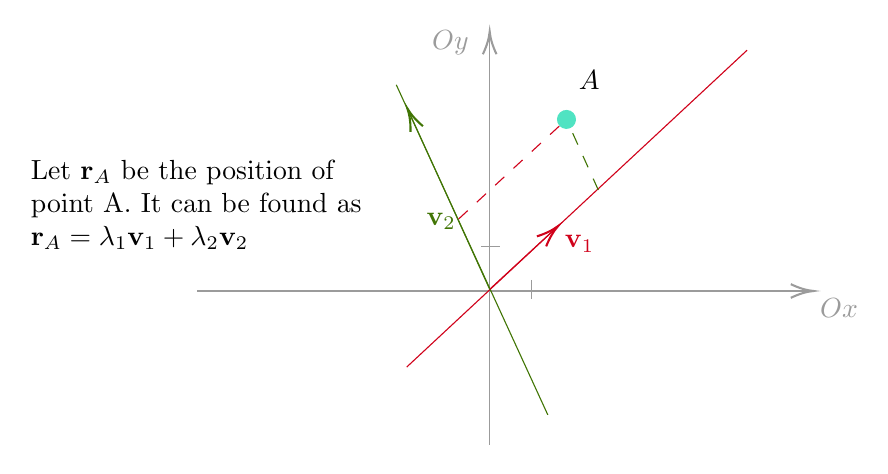
\begin{tikzpicture}[x=0.75pt,y=0.75pt,yscale=-1,xscale=1]
			%uncomment if require: \path (0,300); %set diagram left start at 0, and has height of 300
			
			%Straight Lines [id:da03963288748552296] 
			\draw [color={rgb, 255:red, 155; green, 155; blue, 155 }  ,draw opacity=1 ]   (260,205.5) -- (260,8.33) ;
			\draw [shift={(260,6.33)}, rotate = 90] [color={rgb, 255:red, 155; green, 155; blue, 155 }  ,draw opacity=1 ][line width=0.75]    (10.93,-3.29) .. controls (6.95,-1.4) and (3.31,-0.3) .. (0,0) .. controls (3.31,0.3) and (6.95,1.4) .. (10.93,3.29)   ;
			%Straight Lines [id:da9898822166885091] 
			\draw [color={rgb, 255:red, 155; green, 155; blue, 155 }  ,draw opacity=1 ]   (119,131.33) -- (414,131.33) ;
			\draw [shift={(416,131.33)}, rotate = 180] [color={rgb, 255:red, 155; green, 155; blue, 155 }  ,draw opacity=1 ][line width=0.75]    (10.93,-3.29) .. controls (6.95,-1.4) and (3.31,-0.3) .. (0,0) .. controls (3.31,0.3) and (6.95,1.4) .. (10.93,3.29)   ;
			%Straight Lines [id:da1995149828845848] 
			\draw [color={rgb, 255:red, 208; green, 2; blue, 27 }  ,draw opacity=1 ]   (220,168) -- (384,15.33) ;
			%Straight Lines [id:da3869698901050138] 
			\draw [color={rgb, 255:red, 65; green, 117; blue, 5 }  ,draw opacity=1 ]   (288,191) -- (215,32) ;
			%Straight Lines [id:da1919377633607524] 
			\draw [color={rgb, 255:red, 155; green, 155; blue, 155 }  ,draw opacity=1 ]   (256,110) -- (265,110) ;
			%Straight Lines [id:da10953300738059357] 
			\draw [color={rgb, 255:red, 155; green, 155; blue, 155 }  ,draw opacity=1 ]   (280,126) -- (280,135) ;
			%Straight Lines [id:da23550777917390864] 
			\draw [color={rgb, 255:red, 208; green, 2; blue, 27 }  ,draw opacity=1 ]   (260,130.5) -- (291.53,101.36) ;
			\draw [shift={(293,100)}, rotate = 137.25] [color={rgb, 255:red, 208; green, 2; blue, 27 }  ,draw opacity=1 ][line width=0.75]    (10.93,-3.29) .. controls (6.95,-1.4) and (3.31,-0.3) .. (0,0) .. controls (3.31,0.3) and (6.95,1.4) .. (10.93,3.29)   ;
			%Straight Lines [id:da2310422637940801] 
			\draw [color={rgb, 255:red, 65; green, 117; blue, 5 }  ,draw opacity=1 ]   (260,130.5) -- (221.16,45.15) ;
			\draw [shift={(220.33,43.33)}, rotate = 65.53] [color={rgb, 255:red, 65; green, 117; blue, 5 }  ,draw opacity=1 ][line width=0.75]    (10.93,-3.29) .. controls (6.95,-1.4) and (3.31,-0.3) .. (0,0) .. controls (3.31,0.3) and (6.95,1.4) .. (10.93,3.29)   ;
			%Straight Lines [id:da6904020998642777] 
			\draw [color={rgb, 255:red, 208; green, 2; blue, 27 }  ,draw opacity=1 ] [dash pattern={on 4.5pt off 4.5pt}]  (245,96.67) -- (297,48.67) ;
			%Straight Lines [id:da1717268961570897] 
			\draw [color={rgb, 255:red, 65; green, 117; blue, 5 }  ,draw opacity=1 ] [dash pattern={on 4.5pt off 4.5pt}]  (312.33,82.67) -- (297,48.67) ;
			%Shape: Circle [id:dp39883151826301355] 
			\draw  [color={rgb, 255:red, 80; green, 227; blue, 194 }  ,draw opacity=1 ][fill={rgb, 255:red, 80; green, 227; blue, 194 }  ,fill opacity=1 ] (292.69,48.49) .. controls (292.79,46.11) and (294.8,44.26) .. (297.18,44.36) .. controls (299.56,44.46) and (301.41,46.47) .. (301.31,48.85) .. controls (301.21,51.23) and (299.2,53.07) .. (296.82,52.97) .. controls (294.44,52.87) and (292.59,50.87) .. (292.69,48.49) -- cycle ;
			
			% Text Node
			\draw (418,133.73) node [anchor=north west][inner sep=0.75pt]  [color={rgb, 255:red, 155; green, 155; blue, 155 }  ,opacity=1 ]  {$Ox$};
			% Text Node
			\draw (231,4.73) node [anchor=north west][inner sep=0.75pt]  [color={rgb, 255:red, 155; green, 155; blue, 155 }  ,opacity=1 ]  {$Oy$};
			% Text Node
			\draw (37.67,67) node [anchor=north west][inner sep=0.75pt]   [align=left] {Let $\mathbf r_A$ be the position of \\point A. It can be found as\\ $\mathbf r_A = \lambda_1 \mathbf v_1 + \lambda_2 \mathbf v_2$};
			% Text Node
			\draw (301.67,24.07) node [anchor=north west][inner sep=0.75pt]    {$A$};
			% Text Node
			\draw (295,103.4) node [anchor=north west][inner sep=0.75pt]  [color={rgb, 255:red, 208; green, 2; blue, 27 }  ,opacity=1 ]  {$\mathbf v_{1}$};
			% Text Node
			\draw (228.33,92.73) node [anchor=north west][inner sep=0.75pt]  [color={rgb, 255:red, 65; green, 117; blue, 5 }  ,opacity=1 ]  {$\mathbf v_{2}$};
			
			
		\end{tikzpicture}
		
		
	\end{flushleft}
\end{frame}





\begin{frame}{Span}
	% \framesubtitle{Part 1}
	\begin{flushleft}
		
	Let us examine the equation $\mathbf r_A = \lambda_1 \mathbf v_1 + \lambda_2 \mathbf v_2$ more carefully. First, we can re-write in in matrix form:
	
	\begin{equation}
		\begin{bmatrix}
			\mathbf v_1 & \mathbf v_2
		\end{bmatrix}
		\begin{bmatrix}
			\lambda_1 \\ \lambda_2
		\end{bmatrix}
		=
		\mathbf r_A
	\end{equation}

\bigskip	

	And we know how to solve it. Denoting the matrix $\mathbf M = \begin{bmatrix}
		\mathbf v_1 & \mathbf v_2
	\end{bmatrix}$, we can say that as long as $\mathbf M$ is full rank, the system can be solved exactly. And $\mathbf M$ is full rank, as long as $\mathbf v_1$ and $\mathbf v_2$ are linearly independent.

\bigskip	

	We can call $\lambda_1$ and $\lambda_2$ \emph{coordinates} of $\mathbf r_A$ in the \emph{basis} $\mathbf v_1$ and $\mathbf v_2$.

		
	\end{flushleft}
\end{frame}






\begin{frame}{Span}
	% \framesubtitle{Part 1}
	\begin{flushleft}
		
		If  $\mathbf M = \begin{bmatrix}
			\mathbf v_1 & \mathbf v_2
		\end{bmatrix}$ is full rank, we say that it \emph{spans the plane}. That simply means - any point on the plane can be expressed by its coordinates $\lambda_1$ and $\lambda_2$.
		
		\bigskip	
		
		If you know coordinates $\lambda_1$ and $\lambda_2$ of a point $B$, you can find its position:
		
	\begin{equation}
		\mathbf r_B
		=
	\lambda_1 \mathbf v_1 + \lambda_2 \mathbf v_2
\end{equation}	


If we want to check if two vectors in $\mathbb{R}^2$ are not parallel (are linearly independent), we can see if the following determinant $\Delta$ is not zero:

	\begin{equation}
		\Delta = 
		\text{det}\left(
		\begin{bmatrix}
			\mathbf v_1 & \mathbf v_2
		\end{bmatrix}\right)
\end{equation}	

		
	\end{flushleft}
\end{frame}





\begin{frame}{Dot product}
	% \framesubtitle{Part 1}
	\begin{flushleft}
		
		Given two vectors $\mathbf a = [a_x \ a_y]$ and $\mathbf b = [b_x \ b_y]$, you can define their dot product as:
		
			\begin{equation}
			\mathbf a \cdot \mathbf b = a_x b_x + a_y b_y
		\end{equation}	
	
	\bigskip
		
		We can also define dot product as follows: 
		
		\begin{equation}
			\mathbf a \cdot \mathbf b = 
			||\mathbf a|| \ ||\mathbf b|| \ \text{cos}(\varphi)
		\end{equation}	

	where $\varphi$ is the angle between the two vectors. The two definitions can be used to compute the angle between vectors:
	
		\begin{equation}
			\text{cos}(\varphi) = 
			\frac{\mathbf a \cdot \mathbf b}{||\mathbf a|| \ ||\mathbf b||}
		\end{equation}	
		
	\end{flushleft}
\end{frame}



\begin{frame}{Dot product}
	% \framesubtitle{Part 1}
	\begin{flushleft}
		
		Some examples. If $\mathbf a = [1 \ 0]$ and $\mathbf b = [0 \ 2]$, you can find their dot product as $\mathbf a \cdot \mathbf b = 1 \cdot 0 + 0 \cdot 2 = 0$.

	Meaning the angle between the two vectors is:
	%
	\begin{equation}
		\text{cos}(\varphi) = 
		\frac{0}{1 \cdot 2} = 0, \ \ \ \varphi = \pi/2
	\end{equation}	

\bigskip

If $\mathbf a = [1 \ 1]$ and $\mathbf b = [-2 \ 0]$, their dot product is:
%
\begin{equation}
	\mathbf a \cdot \mathbf b = 1 \cdot (-2) + 1 \cdot 0 = -2
\end{equation}	
%
The angle between the two vectors is:
%
\begin{equation}
	\text{cos}(\varphi) = 
	\frac{-2}{\sqrt{2} \cdot 2} = -\sqrt{2} / 2, \ \ \ \varphi = 3\pi/4
\end{equation}	
		
	\end{flushleft}
\end{frame}




\begin{frame}{Orthogonality}
	% \framesubtitle{Part 1}
	\begin{flushleft}
		
		Given one line, how do we find another, perpendicular (\emph{orthogonal}) to it?
		
		\bigskip
		
		Given one vector, how do we find another, perpendicular to it? Well, by a reasonable definition, two orthogonal vectors would have angle $\varphi = \pi/2$ between them. So, if If $\mathbf a$ and $\mathbf b$ are orthogonal, their dot product is:
		
		\begin{equation}
			\mathbf a \cdot \mathbf b = 
			||\mathbf a|| \ ||\mathbf b|| \ \text{cos}(\pi/2) = 0
		\end{equation}	
		
		Which in turn means:
		
		\begin{equation}
			a_x b_x + a_y b_y = 0
		\end{equation}	
		
	\end{flushleft}
\end{frame}


\begin{frame}{Orthogonality}
% \framesubtitle{Part 1}
\begin{flushleft}
	
	Consider the following problem. Given vector $\mathbf r = [r_x \ r_y]$, find vector $\mathbf n = [n_x \ n_y]$, orthogonal to it.
	
	\bigskip
	
	We know that their dot product has to be zero:
	
	\begin{equation}
		r_x n_x + r_y n_y = 0
	\end{equation}	

	We can rewrite it in matrix form:
	
	
	\begin{equation}
		\begin{bmatrix}
			r_x & r_y
		\end{bmatrix}
		\begin{bmatrix}
		n_x \\ n_y
		\end{bmatrix} = 0
	\end{equation}

\begin{equation}
\mathbf r^\top
\mathbf n = 0
\end{equation}	
	
Meaning we can find $\mathbf n$	using \texttt{lstsq}.
	
	
\end{flushleft}
\end{frame}




\begin{frame}{Orthogonality}
	% \framesubtitle{Part 1}
	\begin{flushleft}
		
		We could find $\mathbf n$ using \texttt{lstsq}. But it looks too complicated for such a simple task.
		
		\bigskip
		
		 Alternatively, we can consider $r_x n_x + r_y n_y = 0$. From this, $n_y = -\frac{r_x}{r_y} n_x$. So, for example, vector $\mathbf n = [1 \ -\frac{r_x}{r_y}]$ is orthogonal to $\mathbf r$.
		 
		 Note that in any case, we can decide we want $\mathbf n$ to have certain lengths, let us say $||\mathbf n|| = 1$. To achieve that we can \emph{normalize} it:
		 
		 \begin{align}
		 	\mathbf n^* = 
		 	\begin{bmatrix}
		 		1 \\ -r_x / r_y
		 	\end{bmatrix}\\
		 	\mathbf n = \frac{\mathbf n^*}{||\mathbf n^*||}
		 \end{align}
		
		
	\end{flushleft}
\end{frame}



\begin{frame}{Affine lines}
	% \framesubtitle{Part 1}
	\begin{flushleft}
		
		If a line does not cross the origin, its equation would have the \emph{affine} form $y = ax + b$:
		
		\bigskip
		
		\tikzset{every picture/.style={line width=0.75pt}} %set default line width to 0.75pt        
		
		\begin{tikzpicture}[x=0.75pt,y=0.75pt,yscale=-1,xscale=1]
			%uncomment if require: \path (0,300); %set diagram left start at 0, and has height of 300
			
			%Straight Lines [id:da14992123684421776] 
			\draw [color={rgb, 255:red, 155; green, 155; blue, 155 }  ,draw opacity=1 ]   (260,205.5) -- (260,8.33) ;
			\draw [shift={(260,6.33)}, rotate = 90] [color={rgb, 255:red, 155; green, 155; blue, 155 }  ,draw opacity=1 ][line width=0.75]    (10.93,-3.29) .. controls (6.95,-1.4) and (3.31,-0.3) .. (0,0) .. controls (3.31,0.3) and (6.95,1.4) .. (10.93,3.29)   ;
			%Straight Lines [id:da6773357142824759] 
			\draw [color={rgb, 255:red, 155; green, 155; blue, 155 }  ,draw opacity=1 ]   (119,130.33) -- (414,130.33) ;
			\draw [shift={(416,130.33)}, rotate = 180] [color={rgb, 255:red, 155; green, 155; blue, 155 }  ,draw opacity=1 ][line width=0.75]    (10.93,-3.29) .. controls (6.95,-1.4) and (3.31,-0.3) .. (0,0) .. controls (3.31,0.3) and (6.95,1.4) .. (10.93,3.29)   ;
			%Straight Lines [id:da8665358232427451] 
			\draw [color={rgb, 255:red, 208; green, 2; blue, 27 }  ,draw opacity=1 ]   (220,169) -- (357,39.5) ;
			%Straight Lines [id:da39036513276793583] 
			\draw [color={rgb, 255:red, 65; green, 117; blue, 5 }  ,draw opacity=1 ]   (203,127.5) -- (260.26,73.35) -- (310,25.5) ;
			%Straight Lines [id:da7101845796956183] 
			\draw [color={rgb, 255:red, 155; green, 155; blue, 155 }  ,draw opacity=1 ]   (256,110) -- (265,110) ;
			%Straight Lines [id:da13284289284233974] 
			\draw [color={rgb, 255:red, 155; green, 155; blue, 155 }  ,draw opacity=1 ]   (280,126) -- (280,135) ;
			%Straight Lines [id:da9183296546556854] 
			\draw [color={rgb, 255:red, 208; green, 2; blue, 27 }  ,draw opacity=1 ]   (260,130.5) -- (291.53,101.36) ;
			\draw [shift={(293,100)}, rotate = 137.25] [color={rgb, 255:red, 208; green, 2; blue, 27 }  ,draw opacity=1 ][line width=0.75]    (10.93,-3.29) .. controls (6.95,-1.4) and (3.31,-0.3) .. (0,0) .. controls (3.31,0.3) and (6.95,1.4) .. (10.93,3.29)   ;
			%Straight Lines [id:da4578798693285282] 
			\draw [color={rgb, 255:red, 65; green, 117; blue, 5 }  ,draw opacity=1 ]   (260.26,73.35) -- (283.69,50.81) ;
			\draw [shift={(285.13,49.43)}, rotate = 136.11] [color={rgb, 255:red, 65; green, 117; blue, 5 }  ,draw opacity=1 ][line width=0.75]    (10.93,-3.29) .. controls (6.95,-1.4) and (3.31,-0.3) .. (0,0) .. controls (3.31,0.3) and (6.95,1.4) .. (10.93,3.29)   ;
			%Straight Lines [id:da4317564949494017] 
			\draw    (260.26,73.35) -- (260.01,128.5) ;
			\draw [shift={(260,130.5)}, rotate = 270.26] [color={rgb, 255:red, 0; green, 0; blue, 0 }  ][line width=0.75]    (10.93,-3.29) .. controls (6.95,-1.4) and (3.31,-0.3) .. (0,0) .. controls (3.31,0.3) and (6.95,1.4) .. (10.93,3.29)   ;
			%Straight Lines [id:da6452459623922309] 
			\draw    (260,130.5) -- (260.25,75.35) ;
			\draw [shift={(260.26,73.35)}, rotate = 90.26] [color={rgb, 255:red, 0; green, 0; blue, 0 }  ][line width=0.75]    (10.93,-3.29) .. controls (6.95,-1.4) and (3.31,-0.3) .. (0,0) .. controls (3.31,0.3) and (6.95,1.4) .. (10.93,3.29)   ;
			
			% Text Node
			\draw (370,34.73) node [anchor=north west][inner sep=0.75pt]  [color={rgb, 255:red, 208; green, 2; blue, 27 }  ,opacity=1 ]  {$y\ =\ ax$};
			% Text Node
			\draw (296,3.4) node [anchor=north west][inner sep=0.75pt]  [color={rgb, 255:red, 65; green, 117; blue, 5 }  ,opacity=1 ]  {$y\ =\ ax+b$};
			% Text Node
			\draw (418,133.73) node [anchor=north west][inner sep=0.75pt]  [color={rgb, 255:red, 155; green, 155; blue, 155 }  ,opacity=1 ]  {$Ox$};
			% Text Node
			\draw (231,4.73) node [anchor=north west][inner sep=0.75pt]  [color={rgb, 255:red, 155; green, 155; blue, 155 }  ,opacity=1 ]  {$Oy$};
			% Text Node
			\draw (95,40) node [anchor=north west][inner sep=0.75pt]   [align=left] {If $\displaystyle x=0$, then $\displaystyle y=b$.};
			% Text Node
			\draw (265,85.4) node [anchor=north west][inner sep=0.75pt]    {$b$};
			
			
		\end{tikzpicture}
		
		
		
	\end{flushleft}
\end{frame}




\begin{frame}{Affine lines}
	% \framesubtitle{Part 1}
	\begin{flushleft}
		
		
		Consider the problem: find a line $\mathcal{L}$ that is $h$-distance away from the line $y = ax$:
		
		\bigskip
		
		
		\tikzset{every picture/.style={line width=0.75pt}} %set default line width to 0.75pt        
		
		\begin{tikzpicture}[x=0.75pt,y=0.75pt,yscale=-1,xscale=1]
			%uncomment if require: \path (0,300); %set diagram left start at 0, and has height of 300
			
			%Straight Lines [id:da8813058365924902] 
			\draw [color={rgb, 255:red, 155; green, 155; blue, 155 }  ,draw opacity=1 ]   (260,205.5) -- (260,8.33) ;
			\draw [shift={(260,6.33)}, rotate = 90] [color={rgb, 255:red, 155; green, 155; blue, 155 }  ,draw opacity=1 ][line width=0.75]    (10.93,-3.29) .. controls (6.95,-1.4) and (3.31,-0.3) .. (0,0) .. controls (3.31,0.3) and (6.95,1.4) .. (10.93,3.29)   ;
			%Straight Lines [id:da2410500416097643] 
			\draw [color={rgb, 255:red, 155; green, 155; blue, 155 }  ,draw opacity=1 ]   (119,130.33) -- (414,130.33) ;
			\draw [shift={(416,130.33)}, rotate = 180] [color={rgb, 255:red, 155; green, 155; blue, 155 }  ,draw opacity=1 ][line width=0.75]    (10.93,-3.29) .. controls (6.95,-1.4) and (3.31,-0.3) .. (0,0) .. controls (3.31,0.3) and (6.95,1.4) .. (10.93,3.29)   ;
			%Straight Lines [id:da7623405600908828] 
			\draw [color={rgb, 255:red, 208; green, 2; blue, 27 }  ,draw opacity=1 ]   (220,169) -- (357,39.5) ;
			%Straight Lines [id:da07610451332287482] 
			\draw [color={rgb, 255:red, 65; green, 117; blue, 5 }  ,draw opacity=1 ]   (203,127.5) -- (260.26,73.35) -- (310,25.5) ;
			%Straight Lines [id:da0925557352066324] 
			\draw [color={rgb, 255:red, 155; green, 155; blue, 155 }  ,draw opacity=1 ]   (256,110) -- (265,110) ;
			%Straight Lines [id:da09702385780953215] 
			\draw [color={rgb, 255:red, 155; green, 155; blue, 155 }  ,draw opacity=1 ]   (280,126) -- (280,135) ;
			%Straight Lines [id:da5080646935233879] 
			\draw [color={rgb, 255:red, 208; green, 2; blue, 27 }  ,draw opacity=1 ]   (260,130.5) -- (291.53,101.36) ;
			\draw [shift={(293,100)}, rotate = 137.25] [color={rgb, 255:red, 208; green, 2; blue, 27 }  ,draw opacity=1 ][line width=0.75]    (10.93,-3.29) .. controls (6.95,-1.4) and (3.31,-0.3) .. (0,0) .. controls (3.31,0.3) and (6.95,1.4) .. (10.93,3.29)   ;
			%Straight Lines [id:da4997231835361593] 
			\draw [color={rgb, 255:red, 65; green, 117; blue, 5 }  ,draw opacity=1 ]   (236,96.5) -- (275.55,58.88) ;
			\draw [shift={(277,57.5)}, rotate = 136.43] [color={rgb, 255:red, 65; green, 117; blue, 5 }  ,draw opacity=1 ][line width=0.75]    (10.93,-3.29) .. controls (6.95,-1.4) and (3.31,-0.3) .. (0,0) .. controls (3.31,0.3) and (6.95,1.4) .. (10.93,3.29)   ;
			%Straight Lines [id:da22745511298010768] 
			\draw    (236,96.5) -- (258.85,128.87) ;
			\draw [shift={(260,130.5)}, rotate = 234.78] [color={rgb, 255:red, 0; green, 0; blue, 0 }  ][line width=0.75]    (10.93,-3.29) .. controls (6.95,-1.4) and (3.31,-0.3) .. (0,0) .. controls (3.31,0.3) and (6.95,1.4) .. (10.93,3.29)   ;
			%Straight Lines [id:da9582807647646359] 
			\draw    (260,130.5) -- (237.15,98.13) ;
			\draw [shift={(236,96.5)}, rotate = 54.78] [color={rgb, 255:red, 0; green, 0; blue, 0 }  ][line width=0.75]    (10.93,-3.29) .. controls (6.95,-1.4) and (3.31,-0.3) .. (0,0) .. controls (3.31,0.3) and (6.95,1.4) .. (10.93,3.29)   ;
			
			% Text Node
			\draw (365,35.73) node [anchor=north west][inner sep=0.75pt]  [color={rgb, 255:red, 208; green, 2; blue, 27 }  ,opacity=1 ]  {$y\ =\ ax$};
			% Text Node
			\draw (296,3.4) node [anchor=north west][inner sep=0.75pt]  [color={rgb, 255:red, 65; green, 117; blue, 5 }  ,opacity=1 ]  {$y\ =\ ax+b$};
			% Text Node
			\draw (418,133.73) node [anchor=north west][inner sep=0.75pt]  [color={rgb, 255:red, 155; green, 155; blue, 155 }  ,opacity=1 ]  {$Ox$};
			% Text Node
			\draw (231,4.73) node [anchor=north west][inner sep=0.75pt]  [color={rgb, 255:red, 155; green, 155; blue, 155 }  ,opacity=1 ]  {$Oy$};
			% Text Node
			\draw (229,109.4) node [anchor=north west][inner sep=0.75pt]    {$h$};
			% Text Node
			\draw (303,98.73) node [anchor=north west][inner sep=0.75pt]  [color={rgb, 255:red, 208; green, 2; blue, 27 }  ,opacity=1 ]  {$v\ =\ [ v_{x} ,\ v_{y}]$};
			
			
		\end{tikzpicture}
		
		
	\end{flushleft}
\end{frame}




\begin{frame}{Affine lines}
	% \framesubtitle{Part 1}
	\begin{flushleft}
		
		The line $\mathcal{L}$ is given by its equation $y = ax +b$. All we need to do is to find $b$, since $a$ is already known. Here is one way to solve it:
		
		\bigskip
		
		\begin{itemize}
			\item Find $\mathbf v$ on the line $y = ax$; $\mathbf v = [1, \ a]$.
			\item Find $\mathbf n$ orthogonal to $\mathbf v$, $||\mathbf n|| = 1$ (see previous slides).
			\item Point $h \mathbf n = [h n_x, \ h n_y]$ lies on $\mathcal{L}$, so $h n_y = a h n_x + b$.
			\item From this, we know that $b = h(n_y - a n_x)$. Done.
		\end{itemize}
		
		\bigskip
		
		Too many steps for such a simple problem? Maybe. But - it is hard to make a mistake doing it this way.
		
	\end{flushleft}
\end{frame}




%\begin{frame}{Read more}
%
%\begin{itemize}
%\item \bref{https://mathinsight.org/matrices_determinants_multivariable_calculus}{mathinsight.org/matrices\_determinants}
%
%\item \bref{https://en.wikipedia.org/wiki/Determinant}{en.wikipedia.org/wiki/Determinant}
%
%\end{itemize}
%
%\end{frame}



\begin{frame}{Thank you!}
\centerline{Lecture slides are available via Moodle.}
\bigskip
\centerline{You can help improve these slides at:}
\centerline{\mygit}
\bigskip
\centerline{Check Moodle for additional links, videos, textbook suggestions.}
\bigskip

\centerline{\textcolor{black}{\qrcode[height=1.6in]{https://github.com/SergeiSa/Extra-math-for-high-school}}}

\end{frame}

\end{document}
